%% module.tex
%
% An Adventure Module class for LaTeX: Example template
%
% Copyright 2016 Michael C. Davis
%
% LICENSE FOR THE WORK
%
% This work consists of the following files:
%    module.cls
%    basic_stats.sty
%    module.tex
%
% This work may be distributed and/or modified under the conditions of the LaTeX
% Project Public License, either version 1.3 of this license or (at your option)
% any later version. The latest version of this license can be found at:
% http://www.latex-project.org/lppl.txt
% and version 1.3 or later is part of all distributions of LaTeX version
% 2005/12/01 or later.
%
% This work has the LPPL maintenance status `author-maintained'.
% 
% The Author and Maintainer of this work is Michael C. Davis
%
%
% LICENSE FOR COMPILED WORKS
%
% You may distribute compiled works generated using the work as specified in
% Clause 3 of the LaTeX Project Public License. If you incorporate Open Gaming
% Content into the compiled work, you must also comply with the terms of that
% license.

\documentclass[a4paper,serif]{module}       % You can choose "letterpaper" or "a4paper" paper sizes
                                            % You can choose "serif" or "sansserif" fonts

% In a future version, it will also be possible to select a different format for stat blocks. In this
% version, only one stat block style (basic) is defined, and it is the default, so no need to select anything.

\usepackage{lipsum}                         % generates filler text, not needed in a real project



\begin{document}

% If you want a title page, the minimum requirement is to define author and title, then use \maketitle

\title{Dungeon Module X2$\varepsilon$\\
An Adventure Module Class and Template}

\author{Michael C. Davis}

% The other title page elements are optional

\subtitle{Introductory module for character levels 1--3}

\coverimage{module_art_cover.png}

\abstract{This template is inspired by the old-school modules of the 1980s. It is an attempt to recapture the look and feel
of those classic adventures using the power and beauty of the \LaTeX~typesetting system. The template is designed to allow
authors to typeset their adventures with a minimum of effort. Write your adventure, add some simple markup notation as shown
in the example file, and in a few clicks you will have a beautifully-formatted PDF.}

\copyrightblock{The \LaTeX~module class is Copyright \copyright 2016 Michael Davis and is distributed under the terms
of the \href{http://www.latex-project.org/lppl.txt}{LaTeX Project Public License} (LPPL) Version 1.3c. You are free to use this
template to generate works for distribution, both for free and commercially, as detailed in Clause 3 of the license.

Some parts of the template are Copyright \copyright 2000--2003 Wizards of the Coast and are distributed under the
\hyperref[ogl]{Open Game License (OGL)} Version 1.0A. The module class includes macros to make it easy to
add the OGL license text to your own work.

The images and maps in this example template are not covered by the LPPL. See the license for each work.}

% The contact block is to typeset your logo(s), company name and/or contact details. It consists of three columns; you
% can use any or all of them. By default the columns are top-aligned and of equal width, but you can redefine this in the
% optional argument. See the documentation of the LaTeX tabular environment for details.

\contactblock[p{2.9cm} p{5.9cm} p{8.9cm}]{% column 1 : logo
\begin{center}

\includegraphics[width=1.5cm]{module_logo.pdf}
\end{center}
}{% column 2 : empty in this example
}{% column 3 : contact details
\vspace{0.4cm}
\begin{flushright}
The author can be contacted on Dragonsfoot (user:
\href{http://www.dragonsfoot.org/forums/ucp.php?i=pm&mode=compose&u=7317}{slithy}).\\[0.5em]

Support for the module class and this template will be provided on the
\href{http://www.dragonsfoot.org/forums/viewforum.php?f=87}{Dragonsfoot Computer Gaming \& Utilities} forum.
\end{flushright}
}

% Typeset the title page from the elements above. Remove \maketitle if you don't want a title page.

\maketitle



%%%%% Start of Page 1 %%%%%



% Display the title text again at the top of the first column
% Optionally, \showtitle[newtext] uses newtext in place of the previously-defined title

\showtitle

This file is both a short tutorial and example of how to use the module class to typeset your fantasy role-playing game adventure.

\part{Introduction}

This template is provided as a resource for authors of adventure modules for fantasy roleplaying games.
The template requires \LaTeX, a free document preparation system for high-quality typesetting. Unlike a conventional
word processor, the \LaTeX~philosophy is to separate the job of writing content from the job of typesetting it for
publication. The idea is that authors can produce beautifully laid out documents without needing to know anything
about typesetting. It also frees authors from all that fiddly adjusting fonts and resizing images. Another advantage
is that all documents produced using this template will have a similar look and feel, so it's ideal if you want to
publish a series of works.

The first thing you need to be aware of is that LaTeX uses a markup language in order to describe document structure and presentation. What LaTeX does is to convert your source text, combined with the markup, into a high quality document. For the purpose of analogy, web pages work in a similar way: the HTML is used to describe the document, but it is your browser that presents it in its full glory - with different colours, fonts, sizes, etc.

\part{Usage}

% \documentclass[a4paper]{dnd_module}
%
% Accepts 'letter' or 'a4paper' options to specify page size. The amount of text on each page is not changed;
% the only difference between the two options is the size of the top margin and left/right margins. This allows
% module writers to easily create two almost identical PDFs for use in USA and Europe/rest of the world.

\part{A very long section heading that will wrap over several lines}

\section{A very long section heading that will wrap over several lines}

\section*{A very long starred section heading that will wrap over several lines}

\subsection{A very long subsection heading that will wrap over several lines}

\subsubsection{A very long subsubsection heading that will wrap over several lines}

\section{Fonts}

blah blahblah blahblah blahblah blahblah blahblah blahblah blahblah blahblah blahblah blahblah blahblah blahblah blahblah blahblah blahblah blahblah blahblah blahblah blahblah blahblah blahblah blahblah blahblah blahblah blahblah blahblah blahblah blahblah blahblah blahblah blahblah blahblah blah                                 

% Choose \rmdefault to select the serifed font and \sfdefault for a sans-serif font
% If you are using the serifed font, the ITC Souvenir, the font used in the Moldvay Basic rulebook from 1981)

% Note on ITC Souvenir font: This font is not included as part of LaTeX and is a commercial font
% which you must have a license to use. It was bundled with some versions of CorelDraw, which is
% a cheap way to obtain a license.
%
% You need the Adobe Type 1 font definitions (.pfb and .afm files) from CorelDraw and the
% corresponding LaTeX .tfm and .vf files, which are available in the corelpak package on
% CTAN:
%
% https://www.ctan.org/pkg/corelpak
%
% There is also the corelpak-contrib package to help with installation:
%
% https://www.ctan.org/pkg/corelpak-contrib

Test font sizes

{\tiny tiny}
{\scriptsize scriptsize}
{\footnotesize footnotesize}
{\small small}
{\normalsize normalsize}
{\large large}
{\Large Large}
{\LARGE LARGE}
{\huge huge}
{\Huge Huge}

\section{Monster Stat Blocks}

\monster[Octopodes]{octopus}{Octopus}{7|3*|20'/50'|8 legs|1d6 each|F6|6|C}
\monster{platypus}{Platypus}{7|3*|20'/50'|bill|1d4|F6|6|C}

First stat block:
\statblock{kobold}{5}{4,4,3,2,1}
Second stat block:
\statblock{kobold}{1}{3}

You must face the \stats[Kobold King!]{kobold}{1}{4}. 
He is with his \stats[10 bodyguards: ]{kobold}{10}{4 each}

\statblock{harpy}{1}{10}
\statblock{harpy}{3}{24 each}

\statblock{octopus}{1}{10}
\statblock{octopus}{3}{24 each}

\statblock{platypus}{1}{10}
\statblock{platypus}{3}{24 each}

\begin{statblockfreestyle}
Jim the Rogue: leather armour, small fruit knife, S7 I12 W5 D17 C12 Ch15. He can backstab with +4 to hit and double damage. AL C
\end{statblockfreestyle}

\section{Tables}

The module class uses the standard \verb|tabular| environment for tables. You need to specify the horizontal alignment of each column as 
usual. The class provides a \verb|\tableheader| macro which centres the table headings and writes a horizontal rule under each
one. You can redefine the column type for headings: the example below uses the \verb|[b]| option to get bold headings.

\section*{Variable Weapon Damage Table}

\begin{center}
\begin{tabular}{cl}
\tableheader[b]{Damage & Weapon Type}
1-2 (1d2) & Small Fruit Knife\\
1-4 (1d4) & Torch\\
1-6 (1d6) & Hand Axe\\
1-8 (1d8) & Battle Axe\\
1-10 (1d10) & Two-handed sword\\
6-36 (6d6) & Laser Cannon\\
\end{tabular}
\end{center}

\noindent If you need to squeeze wide tables into a text column, you can reduce \verb|\tabcolsep|, which controls the spacing between table columns.

\section*{Character Attacks}

\begin{center}
\addtolength{\tabcolsep}{-4.1pt}
\begin{tabular}{lccccccccccccc}
\tableheader{Attacker's Level & 9 & 8 & 7 & 6 & 5 & 4 & 3 & 2 & 1 & 0 & -1 & -2 & -3}
Normal man & 11 & 12 & 13 & 14 & 15 & 16 & 17 & 18 & 19 & 20 & 20 & 20 & 20\\
1st to 3rd & 10 & 11 & 12 & 13 & 14 & 15 & 16 & 17 & 18 & 19 & 20 & 20 & 20\\
4th + higher & 8 & 9 & 10 & 11 & 12 & 13 & 14 & 15 & 16 & 17 & 18 & 19 & 20\\
\end{tabular}
\addtolength{\tabcolsep}{4.1pt}
\end{center}

\noindent See also: the Wandering Monster table on p.\pageref{wanderingmonsters}.

%%%%% Level One %%%%%

% Float the map on a page on its own

\begin{figure*}[p]
\centering
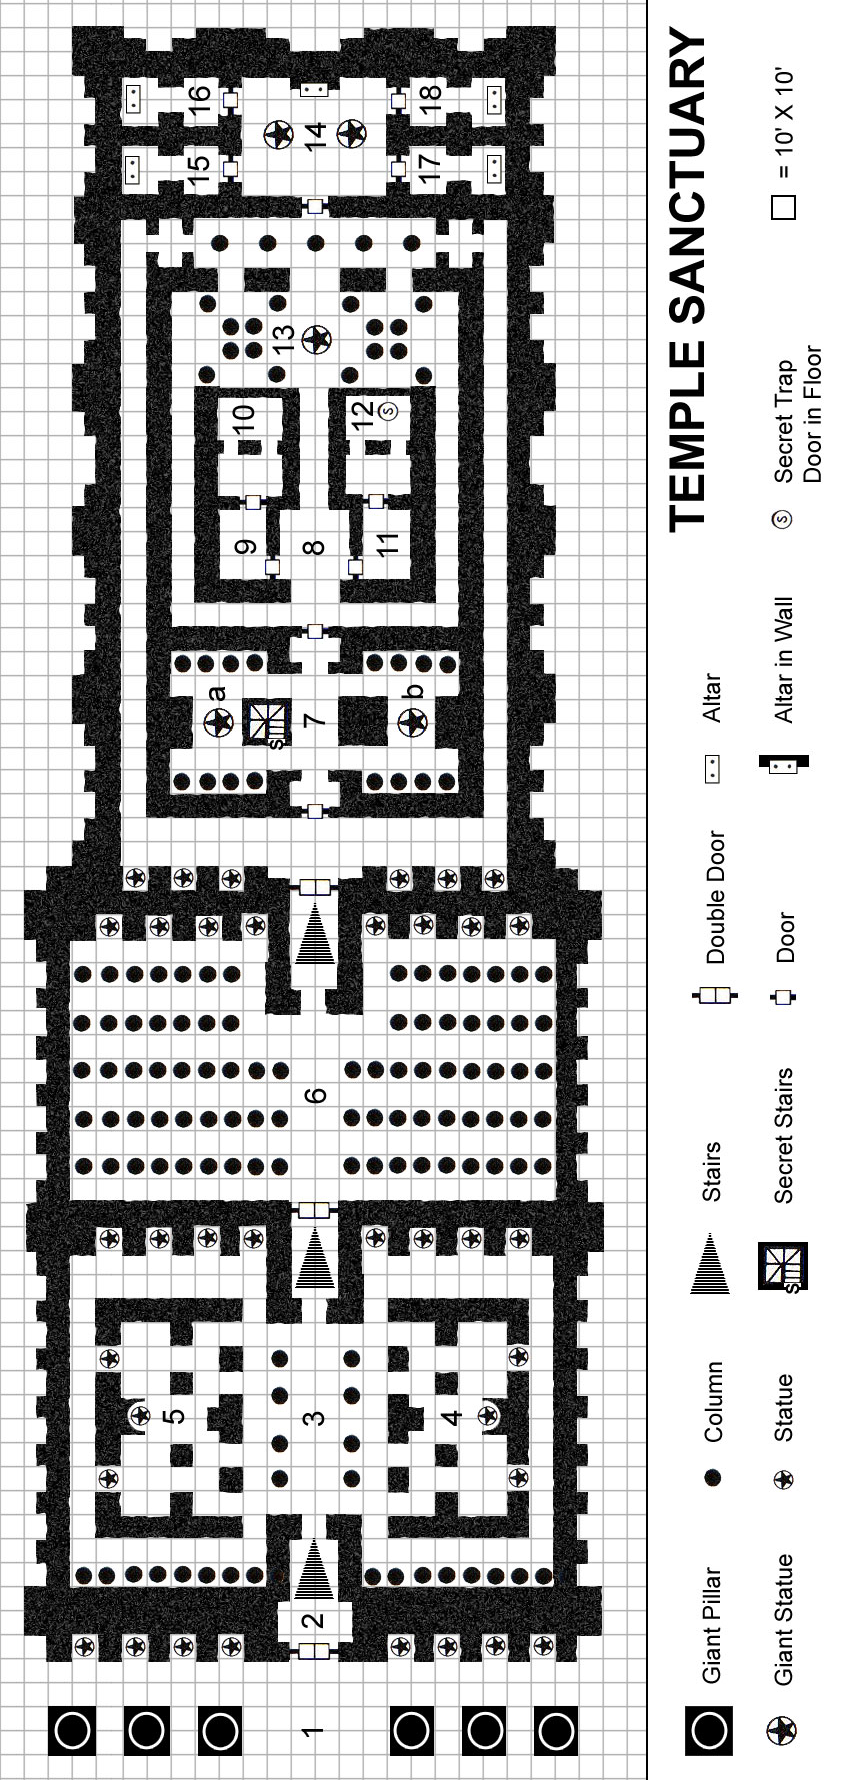
\includegraphics[width=0.75\textwidth]{module_map.png}
\vspace{2em}
\center{Map Copyright \copyright 2008, 2016 Tim Hartin of
\href{http://paratime.ca}{Paratime Design}. Used with permission. All rights reserved.}
\label{img:map}
\end{figure*}

\part{First Dungeon Level}

Some introductory text for the DM.

\section*{Key to Dungeon Level One}

\subsection*{Start}

\boxtext{Some boxed text to read to the players to introduce them to the adventure.}

\subsection{The Gatehouse}

Some DM info above the box blah blah blah blah blah blah blah blah blah blah blah blah blah blah blah blah.

% By default, boxed text is moved up by 0.5em to avoid the space below headings (where it is usually placed)
% being too large. If you want to put a box between normal paragraphs, give it the [0pt] parameter to restore
% the default spacing.

\boxtext[0pt]{It looks dangerous.}

Some monsters are here.
Some DM info below the box blah blah blah blah blah blah blah blah blah blah blah blah blah blah blah blah.

\subsection{The Secret Entrance}

\boxtext{You see some bushes.}

If the players investigate, they will find a hidden trapdoor under the bushes. Under the trapdoor is a tunnel leading under the wall.

\subsection{The big bad end guy}

\begin{figure}[ht]
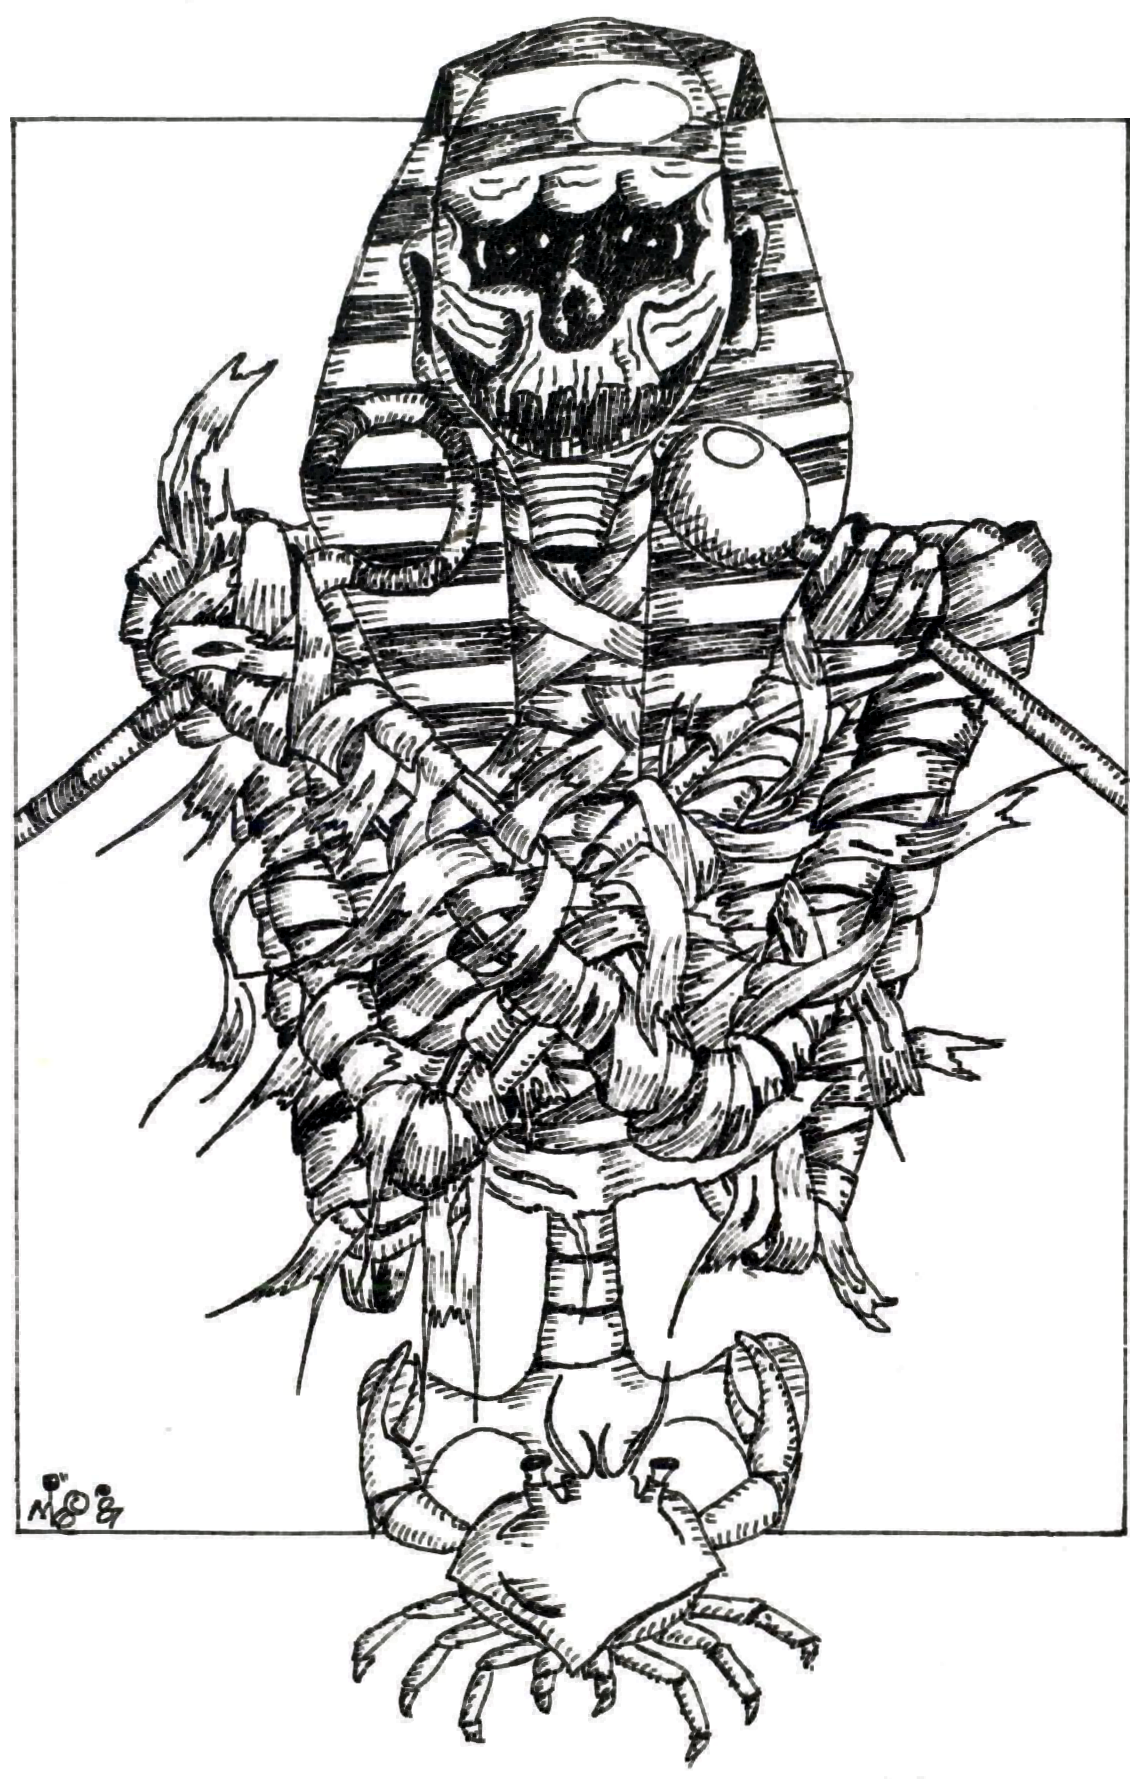
\includegraphics[width=\columnwidth]{module_art_interior.png}
\center{Tomb It May Concern.\\
Image Copyright \copyright 1987, 2016 Michael Davis. All rights reserved.}
\label{img:tomb}
\end{figure}

%%%%% Level Two %%%%%

\begin{table*}[t]
\setlength{\parindent}{1em}
\part{Second Dungeon Level}

If you want to have some pages with a single column of text, you can use \verb|\onecolumn| to switch
into one-column mode and \verb|\twocolumn| to switch back to two-column mode. These commands cause
a page break.

If you want to mix single and double-column text on the same page, use the \verb|table*| environment
to create a float which is the full width of the page. You can do the same thing with graphics using
the \verb|figure*| environment, as we do for the map on p.\pageref{img:map}.

\section*{Wandering Monsters}
\label{wanderingmonsters}

\begin{wanderingmonsters}[b]
1 & Acolyte & 1d8 & 2 & 1 & mace & 1d6 & 60'(20') & C1 & 7 & C\\
2 & Monster with a very long name & 1d8 & 2 & 1 & mace & 1d6 & 60'(20') & C1 & 7 & C\\
\end{wanderingmonsters}

\section*{Monster Roster}

\begin{monsterroster}
1 & Acolyte & 1d8 & 2 & 47 & 1 & mace & 1d6 & 60'(20') & C1 & 7 & C\\
2 & Monster with a very long name & 1d8 & 2 & 23 & 1 & mace & 1d6 & 60'(20') & C1 & 7 & C\\
\end{monsterroster}
\end{table*}

\lipsum

\section{Open Game Content}
\label{ogl}

The template includes macros to make it easy to distribute your work under the Open Game License from Wizards of the Coast.

\begin{ogl}
\item Here include the exact text of the COPYRIGHT NOTICE of any other OGL text you are copying, modifying or distributing.
\item Add the title, copyright date and copyright holder's name(s) of any OGL content you distribute. Example:
\item System Reference Document, Copyright \copyright 2000--2003, Wizards of the Coast, Inc., by Jonathan Tweet, Monte Cook, Skip Williams, Rich Baker, Andy Collins,
David Noonan, Rich Redman, Bruce R. Cordell, John D. Rateliff, Thomas Reid, James Wyatt, based on original material by E. Gary Gygax and Dave Arneson.
\end{ogl}

\begin{productidentity}
\item The text of this \LaTeX~module class and example template, which comprises all typesetting elements and all text which is not explitly Open Game Content, is Product Identity.
\modulecopyright

\item All photographs, artwork and maps in this template are Product Identity.

\item The cover image is adapted from an original image on \href{https://commons.wikimedia.org/wiki/File:Karnak_Tempel_Vorhof_05.jpg}{Wikimedia Commons},
copyright \copyright 2009 Olaf Tausch. Used with permission under the terms of the
\href{https://creativecommons.org/licenses/by/3.0/deed.en}{Creative Commons Attribution 3.0 Unported} license.

\item The map on p.\pageref{img:map} is copyright \copyright 2008, 2016 Tim Hartin of \href{http://paratime.ca}{Paratime Design}. Used with permission. All rights reserved.

\item The drawing on p.\pageref{img:tomb} is copyright \copyright 1987, 2016 Michael Davis. All rights reserved.

\end{productidentity}

\begin{opengamecontent}
\item The monster statistics from the SRD are Open Game Content.
\item The cover page image is in the public domain. The original image is from 
\href{https://commons.wikimedia.org/wiki/File:The_Great_Pyramid_and_the_Sphinx.jpg}{Wikimedia Commons}.
\end{opengamecontent}

% Table of Contents

\tableofcontents

% If you would also like to include an index for your document, see the LaTeX makeidx package

\end{document}
